% ------------------------------------------------------------
% LaTeX Template für die DHBW zum Schnellstart!
% Original: https://github.wdf.sap.corp/vtgermany/LaTeX-Template-DHBW
% ------------------------------------------------------------
% ---- Präambel mit Angaben zum Dokument
\documentclass[
	fontsize=12pt,           % Leitlinien sprechen von Schriftgröße 12.
	paper=A4,
	twoside=false,
	listof=totoc,            % Tabellen- und Abbildungsverzeichnis ins Inhaltsverzeichnis
	bibliography=totoc,      % Literaturverzeichnis ins Inhaltsverzeichnis aufnehmen
	titlepage,               % Titlepage-Umgebung anstatt \maketitle
	headsepline,             % horizontale Linie unter Kolumnentitel
	abstract,              % Überschrift einschalten, Abstract muss in {abstract}-Umgebung stehen
]{scrreprt}                  % Verwendung von KOMA-Report
\usepackage[utf8]{inputenc}  % UTF8 Encoding einschalten
\usepackage[ngerman]{babel}  % Neue deutsche Rechtschreibung
\usepackage[T1]{fontenc}     % Ausgabe von westeuropäischen Zeichen (auch Umlaute)
\usepackage{microtype}       % Trennung von Wörtern wird besser umgesetzt
\usepackage{lmodern}         % Nicht-gerasterte Schriftarten (bei MikTeX erforderlich)
\usepackage{graphicx}        % Einbinden von Grafiken erlauben
\usepackage{wrapfig}         % Grafiken fließend im Text
\usepackage{setspace}        % Zeilenabstand \singlespacing, \onehalfspaceing, \doublespacing
\usepackage[
	%showframe,                % Ränder anzeigen lassen
	left=2.7cm, right=2.5cm,
	top=2.5cm,  bottom=2.5cm,
	includeheadfoot
]{geometry}                      % Seitenlayout einstellen
\usepackage{scrlayer-scrpage}    % Gestaltung von Fuß- und Kopfzeilen
\usepackage{acronym}             % Abkürzungen, Abkürzungsverzeichnis
\usepackage{titletoc}            % Anpassungen am Inhaltsverzeichnis
\contentsmargin{0.75cm}          % Abstand im Inhaltsverzeichnis zw. Punkt und Seitenzahl
\usepackage[                     % Klickbare Links (enth. auch "nameref", "url" Package)
  hidelinks,                     % Blende die "URL Boxen" aus.
  breaklinks=true                % Breche zu lange URLs am Zeilenende um
]{hyperref}
\usepackage[hypcap=true]{caption}% Anker Anpassung für Referenzen
\urlstyle{same}                  % Aktuelle Schrift auch für URLs
% Anpassung von autoref für Gleichungen (ergänzt runde Klammern) und Algorithm.
% Anstatt "Listing" kann auch z.B. "Code-Ausschnitt" verwendet werden. Dies sollte
% jedoch synchron gehalten werden mit \lstlistingname (siehe weiter unten).
\addto\extrasngerman{%
	\def\equationautorefname~#1\null{Gleichung~(#1)\null}
	\def\lstnumberautorefname{Zeile}
	\def\lstlistingautorefname{Listing}
	\def\algorithmautorefname{Algorithmus}
	% Damit einheitlich "Abschnitt 1.2[.3]" verwendet wird und nicht "Unterabschnitt 1.2.3"
	% \def\subsectionautorefname{Abschnitt}
}

% ---- Abstand verkleinern von der Überschrift 
\renewcommand*{\chapterheadstartvskip}{\vspace*{.5\baselineskip}}

% Hierdurch werden Schusterjungen und Hurenkinder vermieden, d.h. einzelne Wörter
% auf der nächsten Seite oder in einer einzigen Zeile.
% LaTeX kann diese dennoch erzeugen, falls das Layout ansonsten nicht umsetzbar ist.
% Diese Werte sind aber gute Startwerte.
\widowpenalty10000
\clubpenalty10000

% ---- Für das Quellenverzeichnis
\usepackage[
	backend = biber,                % Verweis auf biber
	language = auto,
	style = alphabetic,                % Nummerierung der Quellen mit Zahlen
	sorting = anyt,                 % none = Sortierung nach der Erscheinung im Dokument
	sortcites = true,               % Sortiert die Quellen innerhalb eines cite-Befehls
	block = space,                  % Extra Leerzeichen zwischen Blocks
	hyperref = true,                % Links sind klickbar auch in der Quelle
	%backref = true,                % Referenz, auf den Text an die zitierte Stelle
	bibencoding = auto,
	giveninits = true,              % Vornamen werden abgekürzt
	doi=false,                      % DOI nicht anzeigen
	isbn=false,                     % ISBN nicht anzeigen
    alldates=short                  % Datum immer als DD.MM.YYYY anzeigen
]{biblatex}
\addbibresource{Inhalt/literatur.bib}
\setcounter{biburlnumpenalty}{3000}     % Umbruchgrenze für Zahlen
\setcounter{biburlucpenalty}{6000}      % Umbruchgrenze für Großbuchstaben
\setcounter{biburllcpenalty}{9000}      % Umbruchgrenze für Kleinbuchstaben
\DeclareNameAlias{default}{family-given}  % Nachname vor dem Vornamen
\AtBeginBibliography{\renewcommand{\multinamedelim}{\addslash\space
}\renewcommand{\finalnamedelim}{\multinamedelim}}  % Schrägstrich zwischen den Autorennamen
\DefineBibliographyStrings{german}{
  urlseen = {Einsichtnahme:},                      % Ändern des Titels von "besucht am"
}
\usepackage[babel,german=quotes]{csquotes}         % Deutsche Anführungszeichen + Zitate


% ---- Für Mathevorlage
\usepackage{amsmath}    % Erweiterung vom Mathe-Satz
\usepackage{amssymb}    % Lädt amsfonts und weitere Symbole
\usepackage{MnSymbol}   % Für Symbole, die in amssymb nicht enthalten sind.


% ---- Für Quellcodevorlage
\usepackage{scrhack}                    % Hack zur Verw. von listings in KOMA-Script
\usepackage{listings}                   % Darstellung von Quellcode
\usepackage{xcolor}                     % Einfache Verwendung von Farben
% -- Eigene Farben für den Quellcode
\definecolor{JavaLila}{rgb}{0.4,0.1,0.4}
\definecolor{JavaGruen}{rgb}{0.3,0.5,0.4}
\definecolor{JavaBlau}{rgb}{0.0,0.0,1.0}
\definecolor{ABAPKeywordsBlue}{HTML}{6000ff}
\definecolor{ABAPCommentGrey}{HTML}{808080}
\definecolor{ABAPStringGreen}{HTML}{4da619}
\definecolor{PyKeywordsBlue}{HTML}{0000AC}
\definecolor{PyCommentGrey}{HTML}{808080}
\definecolor{PyStringGreen}{HTML}{008080}
% -- Farben für ABAP CDS
\definecolor{CDSString}{HTML}{FF8C00}
\definecolor{CDSKeywords}{HTML}{6000ff}
\definecolor{CDSAnnotation}{HTML}{00BFFF}
\definecolor{CDSComment}{HTML}{808080}
\definecolor{CDSFunc}{HTML}{FF0000}
% -- Farben für SQL
\definecolor{SQLString}{HTML}{15ABF6}
\definecolor{SQLKeywords}{HTML}{7B30FF}
\definecolor{SQLVariables}{HTML}{000000}

% -- Default Listing-Styles

\lstset{
	% Das Paket "listings" kann kein UTF-8. Deswegen werden hier 
	% die häufigsten Zeichen definiert (ä,ö,ü,...)
	literate=%
		{á}{{\'a}}1 {é}{{\'e}}1 {í}{{\'i}}1 {ó}{{\'o}}1 {ú}{{\'u}}1
		{Á}{{\'A}}1 {É}{{\'E}}1 {Í}{{\'I}}1 {Ó}{{\'O}}1 {Ú}{{\'U}}1
		{à}{{\`a}}1 {è}{{\`e}}1 {ì}{{\`i}}1 {ò}{{\`o}}1 {ù}{{\`u}}1
		{À}{{\`A}}1 {È}{{\'E}}1 {Ì}{{\`I}}1 {Ò}{{\`O}}1 {Ù}{{\`U}}1
		{ä}{{\"a}}1 {ë}{{\"e}}1 {ï}{{\"i}}1 {ö}{{\"o}}1 {ü}{{\"u}}1
		{Ä}{{\"A}}1 {Ë}{{\"E}}1 {Ï}{{\"I}}1 {Ö}{{\"O}}1 {Ü}{{\"U}}1
		{â}{{\^a}}1 {ê}{{\^e}}1 {î}{{\^i}}1 {ô}{{\^o}}1 {û}{{\^u}}1
		{Â}{{\^A}}1 {Ê}{{\^E}}1 {Î}{{\^I}}1 {Ô}{{\^O}}1 {Û}{{\^U}}1
		{œ}{{\oe}}1 {Œ}{{\OE}}1 {æ}{{\ae}}1 {Æ}{{\AE}}1 {ß}{{\ss}}1
		{ű}{{\H{u}}}1 {Ű}{{\H{U}}}1 {ő}{{\H{o}}}1 {Ő}{{\H{O}}}1
		{ç}{{\c c}}1 {Ç}{{\c C}}1 {ø}{{\o}}1 {å}{{\r a}}1 {Å}{{\r A}}1
		{€}{{\euro}}1 {£}{{\pounds}}1 {«}{{\guillemotleft}}1
		{»}{{\guillemotright}}1 {ñ}{{\~n}}1 {Ñ}{{\~N}}1 {¿}{{?`}}1,
	breaklines=true,        % Breche lange Zeilen um 
	breakatwhitespace=true, % Wenn möglich, bei Leerzeichen umbrechen
	% Symbol für Zeilenumbruch einfügen
	prebreak=\raisebox{0ex}[0ex][0ex]{\ensuremath{\rhookswarrow}},
	postbreak=\raisebox{0ex}[0ex][0ex]{\ensuremath{\rcurvearrowse\space}},
	tabsize=4,                                 % Setze die Breite eines Tabs
	basicstyle=\ttfamily\small,                % Grundsätzlicher Schriftstyle
	columns=fixed,                             % Besseres Schriftbild
	numbers=left,                              % Nummerierung der Zeilen
	%frame=single,                             % Umrandung des Codes
	showstringspaces=false,                    % Keine Leerzeichen hervorheben
	keywordstyle=\color{blue},
	ndkeywordstyle=\bfseries\color{darkgray},
	identifierstyle=\color{black},
	commentstyle=\itshape\color{JavaGruen},   % Kommentare in eigener Farbe
	stringstyle=\color{JavaBlau},             % Strings in eigener Farbe,
	captionpos=b,                             % Bild*unter*schrift
	xleftmargin=5.0ex
}

% ---- Eigener JAVA-Style für den Quellcode
\renewcommand{\ttdefault}{pcr}               % Schriftart, welche auch fett beinhaltet
\lstdefinestyle{EigenerJavaStyle}{
	language=Java,                             % Syntax Highlighting für Java
	%frame=single,                             % Umrandung des Codes
	keywordstyle=\bfseries\color{JavaLila},    % Keywords in eigener Farbe und fett
	commentstyle=\itshape\color{JavaGruen},    % Kommentare in eigener Farbe und italic
	stringstyle=\color{JavaBlau}               % Strings in eigener Farbe
}

% ---- Eigener ABAP-Style für den Quellcode
\renewcommand{\ttdefault}{pcr}
\lstdefinestyle{EigenerABAPStyle}{
	language=[R/3 6.10]ABAP,
	morestring=[b]\|,                          % Für Pipe-Strings
	morestring=[b]\`,                          % für Backtick-Strings
	keywordstyle=\bfseries\color{ABAPKeywordsBlue},
	commentstyle=\itshape\color{ABAPCommentGrey},
	stringstyle=\color{ABAPStringGreen},
	tabsize=2,
	morekeywords={
		types,
		@data,
		as,
		lower,
		start,
		selection,
		order,
		by,
		inner,
		join,
		key,
		end,
		cast
	}
}

% ---- Eigener SQL-Style für den Quellcode
\renewcommand{\ttdefault}{pcr}
\lstdefinestyle{EigenerSQLStyle}{
	language=SQL,
	keywordstyle=\bfseries\color{SQLKeywords},
	commentstyle=\itshape\color{ABAPCommentGrey},
	stringstyle=\color{SQLString},
	morekeywords={
		SELECT,
		INSERT,
		CREATE,
		UPDATE,
		MOVE,
		AS,
		ON,
		COUNT,
		MAX,
		MIN,
		DELETE,
		GRANT,
		PERMISSIONS,
		ALL,
		REVOKE,
		INNER JOIN,
		RIGHT JOIN,
		LEFT JOIN,
		FULL JOIN,
		FULL OUTER JOIN,
		CROSS JOIN,
		IS,
		NULL,
		DISTINCT,
		JOIN
	}
}

% ---- Eigener Python-Style für den Quellcode
\renewcommand{\ttdefault}{pcr}
\lstdefinestyle{EigenerPythonStyle}{
	language=Python,
	columns=flexible,
	keywordstyle=\bfseries\color{PyKeywordsBlue},
	commentstyle=\itshape\color{PyCommentGrey},
	stringstyle=\color{PyStringGreen}
}

%----- ABAP-CDS-View language
\lstdefinelanguage{ABAPCDS}{
	sensitive=false,
	%Keywords
	morekeywords={define,
		view,
		as,
		select,
		from,
		inner,
		join,
		on,
		key,
		case,
		when,
		then,
		else,
		end,
		true,
		false,
		cast,
		where,
		and,
		distinct,
		group,
		by,
		having,
		min,
		sum,
		max,
		count,
		avg
	},
	%Methoden
	morekeywords=[2]{
		div,
		currency\_conversion,
		dats\_days\_between,
		concat\_with\_space,
		dats\_add_days,
		dats\_is\_valid,
		dats\_add\_months,
		unit\_conversion,
		division,
		mod,
		abs,
		floor,
		ceil,
		round,
		concat,
		replace,
		substring,
		left,
		right,
		length
	},
	morecomment=[s][\color{CDSAnnotation}]{@}{:},
	morecomment=[l][\itshape\color{CDSComment}]{//},
	morecomment=[s][\itshape\color{CDSComment}]{/*}{*/},
	morestring=[b][\color{CDSString}]',
	keywordstyle=\bfseries\color{CDSKeywords},
	keywordstyle=[2]\color{CDSFunc}
}

  % Weitere Details sind ausgelagert

\usepackage{algorithm}                  % Für Algorithmen-Umgebung (ähnlich wie lstlistings Umgebung)
\usepackage{algpseudocode}              % Für Pseudocode. Füge "[noend]" hinzu, wenn du kein "endif",
                                        % etc. haben willst.

\makeatletter                           % Sorgt dafür, dass man @ in Namen verwenden kann.
                                        % Ansonsten gibt es in der nächsten Zeile einen Compilefehler.
\renewcommand{\ALG@name}{Algorithmus}   % Umbenennen von "Algorithm" im Header der Listings.
\makeatother                            % Zeichen wieder zurücksetzen
\renewcommand{\lstlistingname}{Listing} % Erlaubt das Umbenennen von "Listing" in anderen Titel.

% ---- Tabellen
\usepackage{booktabs}  % Für schönere Tabellen. Enthält neue Befehle wie \midrule
\usepackage{multirow}  % Mehrzeilige Tabellen
\usepackage{siunitx}   % Für SI Einheiten und das Ausrichten Nachkommastellen
\sisetup{locale=DE, range-phrase={~bis~}, output-decimal-marker={,}} % Damit ein Komma und kein Punkt verwendet wird.
\usepackage{xfrac} % Für siunitx Option "fraction-function=\sfrac"

% ---- Für Definitionsboxen in der Einleitung
\usepackage{amsthm}                     % Liefert die Grundlagen für Theoreme
\usepackage[framemethod=tikz]{mdframed} % Boxen für die Umrandung
% ---- Definition für Highlight Boxen

% ---- Grundsätzliche Definition zum Style
\newtheoremstyle{defi}
  {\topsep}         % Abstand oben
  {\topsep}         % Abstand unten
  {\normalfont}     % Schrift des Bodys
  {0pt}             % Einschub der ersten Zeile
  {\bfseries}       % Darstellung von der Schrift in der Überschrift
  {:}               % Trennzeichen zwischen Überschrift und Body
  {.5em}            % Abstand nach dem Trennzeichen zum Body Text
  {\thmname{#3}}    % Name in eckigen Klammern
\theoremstyle{defi}

% ------ Definition zum Strich vor eines Texts
\newmdtheoremenv[
  hidealllines = true,       % Rahmen komplett ausblenden
  leftline = true,           % Linie links einschalten
  innertopmargin = 0pt,      % Abstand oben
  innerbottommargin = 4pt,   % Abstand unten
  innerrightmargin = 0pt,    % Abstand rechts
  linewidth = 3pt,           % Linienbreite
  linecolor = gray!40,       % Linienfarbe
]{defStrich}{Definition}     % Name der des formats "defStrich"

% ------ Definition zum Eck-Kasten um einen Text
\newmdtheoremenv[
  hidealllines = true,
  innertopmargin = 6pt,
  linecolor = gray!40,
  singleextra={              % Eck-Markierungen für die Definition
    \draw[line width=3pt,gray!50,line cap=rect] (O|-P) -- +(1cm,0pt);
    \draw[line width=3pt,gray!50,line cap=rect] (O|-P) -- +(0pt,-1cm);
    \draw[line width=3pt,gray!50,line cap=rect] (O-|P) -- +(-1cm,0pt);
    \draw[line width=3pt,gray!50,line cap=rect] (O-|P) -- +(0pt,1cm);
  }
]{defEckKasten}{Definition}  % Name der des formats "defEckKasten"  % Weitere Details sind ausgelagert

% ---- Für Todo Notes
\usepackage{todonotes}
\setlength {\marginparwidth }{2cm}      % Abstand für Todo Notizen

\usepackage{pdfpages}
\usepackage{chngcntr}

% ---- Elektronische Version oder Gedruckte Version?
% ---- Unterschied: Die elektronische Version enthält keinen Platzhalter für die Unterschrift
\usepackage{ifthen}
\newboolean{e-Abgabe}
\setboolean{e-Abgabe}{false}    % false=gedruckte Fassung

% ---- Persönlichen Daten:
\newcommand{\titel}{Untersuchung verschiedener Einsatzmöglichkeiten von Künstlicher Intelligenz bei der Softwareentwicklung im ABAP-Umfeld}
\newcommand{\titelheader}{Künstliche Intelligenz im ABAP-Umfeld}
\newcommand{\arbeit}{Masterarbeit}
\newcommand{\studiengang}{Data Science}
\newcommand{\studienjahr}{2025}
\newcommand{\autor}{Mathis Neunzig}
\newcommand{\autorReverse}{Neunzig, Mathis}
\newcommand{\verfassungsort}{Heidelberg}
\newcommand{\matrikelnr}{XXXXXXX}
\newcommand{\bearbeitungsmonat}{XX - XX 2025}
\newcommand{\abgabe}{XX.XX.2025}
\newcommand{\bearbeitungszeitraum}{XX.XX.2025 - XX.XX.2025}
\newcommand{\fakultaet}{Informatik}
\newcommand{\gutachter}{X}
\newcommand{\zweitgutachter}{X}

% ---- Metainformation für das PDF Dokument
\hypersetup{
	pdftitle    = {\titel},
	pdfsubject  = {\arbeit},
	pdfauthor   = {\autor},
	%pdfkeywords = {Keywords angeben},
	pdfcreator  = {LaTeX},
	%pdfproducer = {in der Regel pdfTeX}
}

% ---- Definition der Kopf- und Fußzeilen
\clearpairofpagestyles                          % Löschen von LaTeX Standard
\automark[section]{chapter}                     % Füllen von section und chapter
\renewcommand*{\chaptermarkformat}{}            % Entfernt die Kapitelnummer
\renewcommand*{\sectionmarkformat}{}            % Entfernt die Sectionnummer
% Angaben [für "plain"]{für "scrheadings"}
\ihead[]{\titelheader}                          % Kopfzeile links
\chead[]{}                                      % Kopfzeile mitte
\ohead[]{\rightmark}                            % Kopfzeile rechts
\ifoot[]{}                                      % Fußzeile links
\cfoot*{\sffamily\pagemark}                     % Fußzeile mitte
\ofoot[]{}                                      % Fußzeile rechts
\KOMAoptions{
   headsepline = 0.2pt,                         % Liniendicke Kopfzeile
   footsepline = false                          % Liniendicke Fußzeile
}


% ---- Hilfreiches
\newcommand{\zB}{z.\,B. }   % "z.B." mit kleinem Leeraum dazwischen (ohne wäre nicht korrekt)
\newcommand{\dash}{d.\,h. }

\newcommand{\code}[1]{\texttt{#1}} % Ist einfacher zu schreiben als ständig \texttt und erlaubt
                                   % Änderungen im Nachhinein, wenn man z.B. Inline-Code anders stylen möchte.

% ---- Silbentrennung (falls LaTeX defaults falsch / nicht gewünscht sind)
\hyphenation{HANA}         % anstatt HA-NA
\hyphenation{Graph-Script} % anstatt GraphS-cript

% ---- Beginn des Dokuments
\begin{document}

\counterwithout{lstlisting}{chapter}
\counterwithout{figure}{chapter}
\counterwithout{table}{chapter}
\setlength{\parindent}{0pt}              % Keine Paragraphen Einrückung.
                                         % Dafür haben wir den Abstand zwischen den Paragraphen.
\setcounter{secnumdepth}{3}              % Nummerierungstiefe fürs Inhaltsverzeichnis
\setcounter{tocdepth}{1}                 % Tiefe des Inhaltsverzeichnisses. Ggf. so anpassen,
                                         % dass das Verzeichnis auf eine Seite passt.
\sffamily                                % Serifenlose Schrift verwenden.


% ---- Vorspann
% ------ Titelseite
\singlespacing
\thispagestyle{empty}
\begin{titlepage}
\enlargethispage{4cm}

\begin{center}
    
\includegraphics[height=2.5cm]{Bilder/Logos/Logo_Uni.png} 
\end{center}
\vspace*{0.1cm}

\begin{center}
	\huge{\textbf{\titel}}\\[1.5cm]
	\Large{\textbf{\arbeit}}\\[0.5cm]
	\normalsize{im Rahmen der Prüfung zum\\[1ex] \textbf{Master of Science (M.Sc.)}}\\[0.5cm]
	\Large{des Studienganges \studiengang}\\[1ex]
	\normalsize{an der FernUniversität in Hagen}\\[1cm]
	\normalsize{von}\\[1ex] \Large{\textbf{\autor}} \\[1cm]
	% Hinweis: Manche Dozenten möchten einen Hinweis auf den Sperrvermerk auf der Titelseite.
	% \large{{\color{red}- Sperrvermerk -}}\\[1cm]
\end{center}

\begin{center}
	\vfill
	\begin{tabular}{ll}
		Abgabedatum:                     & \abgabe \\[0.2cm]
		Bearbeitungszeitraum:            & \bearbeitungszeitraum \\[0.2cm]
		Matrikelnummer:                  & \matrikelnr \\[0.2cm]
		Fakultät:                        & \fakultaet \\[0.2cm]
		Gutachter:                       & \gutachter \\[0.2cm]
		Zweitgutachter:                  & \zweitgutachter \\[2cm]
	\end{tabular} 
\end{center}
\end{titlepage}
  % Titelseite
\newcounter{savepage}
\pagenumbering{Roman}                    % Römische Seitenzahlen
\onehalfspacing

% ------ Erklärung, Sperrvermerk, Abstact, Vorwort
\chapter*{Eidesstattliche Erklärung}
Ich erkläre, dass ich die \arbeit{} mit dem Thema:
\begin{quote}
	\textit{\titel}
\end{quote} 
selbstständig und ohne unzulässige Inanspruchnahme Dritter verfasst habe. Ich habe dabei nur die angegebenen Quellen und Hilfsmittel verwendet und die aus diesen wörtlich oder sinngemäß entnommenen Stellen als solche kenntlich gemacht. Die Versicherung selbstständiger Arbeit gilt auch für enthaltene Zeichnungen, Skizzen oder graphische Darstellungen. Die Arbeit wurde bisher in gleicher oder ähnlicher Form weder derselben noch einer anderen Prüfungsbehörde vorgelegt und auch nicht veröffentlicht. Mit der Abgabe der elektronischen Fassung der endgültigen Version der Arbeit nehme ich zur Kenntnis, dass diese mit Hilfe eines Plagiatserkennungsdienstes auf enthaltene Plagiate geprüft werden kann und ausschließlich für Prüfungszwecke gespeichert wird. Ich versichere zudem, dass die eingereichte elektronische Fassung mit eventuell gedruckt eingereichten Fassungen übereinstimmt.

\vspace{1cm}

\verfassungsort, den \today \\[0.5cm]
\ifthenelse{\boolean{e-Abgabe}}
	{\underline{Gez. \autor}}
	{\makebox[6cm]{\hrulefill}}\\ 
\autorReverse

\renewcommand{\abstractname}{Abstract} % Veränderter Name für das Abstract
\begin{abstract}
\begin{addmargin}[0.5cm]{0.5cm}        % Erhöhte Ränder, für Abstract Look
\thispagestyle{plain}                  % Seitenzahl auf der Abstract Seite

\begin{center}
\small\textit{- English -}             % Angabe der Sprache für das Abstract
\end{center}

\vspace{0.25cm}

Text

\vspace{0.25cm}

Text

\vspace{0.25cm} 

Text

\end{addmargin}
\end{abstract}
\renewcommand{\abstractname}{Abstract} % Veränderter Name für das Abstract
\begin{abstract}
\begin{addmargin}[0.5cm]{0.5cm}        % Erhöhte Ränder, für Abstract Look
\thispagestyle{plain}                  % Seitenzahl auf der Abstract Seite

\begin{center}
\small\textit{- Deutsch -}             % Angabe der Sprache für das Abstract
\end{center}

\vspace{0.25cm}

Text

\vspace{0.25cm}

Text

\vspace{0.25cm} 

Text

\end{addmargin}
\end{abstract}
\chapter*{Vorwort}
%\addcontentsline{toc}{chapter}{Vorwort} % Hinzufügen zum Inhaltsverzeichnis 
\section*{Danksagung}
An dieser Stelle möchte ich mich bei all denjenigen bedanken, die mich während der Anfertigung meiner Masterarbeit unterstützt und motiviert haben.

\vspace{0.25cm}
Fernuni Hagen

\vspace{0.25cm}
SAP Team

\vspace{0.25cm}
SAP Team Special

\vspace{0.25cm}
Familie und Freunde

\section*{Disclaimer}
In dieser Arbeit wird aus Gründen der besseren Lesbarkeit auf die gleichzeitige Verwendung der Sprachformen männlich, weiblich und divers (m/w/d) verzichtet und das generische Maskulinum verwendet. Weibliche und anderweitige Geschlechteridentitäten werden dabei ausdrücklich mitgemeint, soweit es für die Aussage erforderlich ist.

\vspace{0.25cm}
Abbildungen, Codebeispiele und Tabellen, die den Lesefluss stören, befinden sich im Anhang. Ist dies der Fall, wird im Text zusätzlich auf den Anhang verwiesen.

\vspace{0.25cm}
Ein Teil der Literatur, die für die Anfertigung dieser Arbeit genutzt wird, ist nur über die E-Book-Plattform o'Reilly abrufbar. Bei diesen Ressourcen existieren keine Seitennummern, es wird bei Verweisen stattdessen die Kapitelnummer angegeben.

% ------ Inhaltsverzeichnis
\singlespacing
\tableofcontents

% ------ Verzeichnisse
\renewcommand*{\chapterpagestyle}{plain}
\pagestyle{plain}
\chapter*{Abkürzungsverzeichnis}
\addcontentsline{toc}{chapter}{Abkürzungsverzeichnis} % Hinzufügen zum Inhaltsverzeichnis 

\begin{acronym}[WYSISWG] % längstes Kürzel wird verw. für den Abstand zw. Kürzel u. Text

	% Alphabetisch selbst sortieren - nicht verwendete Kürzel rausnehmen!
	\acro{ABAP}{Advanced Business Application Programming}
        \acro{BTP}{Business Technology Platform}

\end{acronym}
\listoffigures                          % Erzeugen des Abbildungsverzeichnisses 
\listoftables                           % Erzeugen des Tabellenverzeichnisses
\renewcommand{\lstlistlistingname}{Quellcodeverzeichnis}
\lstlistoflistings                      % Erzeugen des Listenverzeichnisses
\setcounter{savepage}{\value{page}}


% ---- Inhalt der Arbeit
\cleardoublepage
\pagenumbering{arabic}                  % Arabische Seitenzahlen für den Hauptteil
\setlength{\parskip}{0.5\baselineskip}  % Abstand zwischen Absätzen
\rmfamily
\renewcommand*{\chapterpagestyle}{scrheadings}
\pagestyle{scrheadings}
\onehalfspacing
\chapter{Einleitung}

\section{Motivation}

\section{Problemstellung}

\section{Methodik}

\section{Struktur}

\chapter{Theoretische Grundlagen}
Um den Gedanken in den folgenden Kapiteln folgen zu können, ist es wichtig, vorab Grundbegriffe und Konzepte zu erklären. Diese theoretischen Grundlagen, Grundbegriffe und Konzepte werden in den Folgekapiteln vorgestellt.

\section{Grundbegriffe}
Die folgenden Grundbegriffe sind essenzielle Vokabeln in dieser Masterarbeit und somit zum vollen Verständnis notwendig. Dabei handelt es sich um technische Grundlagen aus dem Umfeld dieser Arbeit sowie die Beschreibung der benutzten Methoden und Softwareprodukte.

\subsection{ABAP}
\ac{ABAP} ist eine domänenspezifische Programmiersprache der 4. Generation \cite[S. 25]{keller_abap_2006}, die 1983 von SAP speziell für die Entwicklung von Geschäftsapplikationen entwickelt wurde und somit in den SAP-Umgebungen genutzt werden kann \cite[S. 1/2ff]{sap-documentation_abap4_1996}. Sie wurde ursprünglich für die Programmierung von R/3-Systemen entwickelt, kann jedoch auch in modernen Produkten und System der SAP genutzt werden \cite[S. 23ff.]{keller_abap_2006}. Dabei ist das dazugehörige R/3-System ein Enterprise-Ressource-Planning-System, welches 1992 von SAP veröffentlicht wurde \cite[S. 15]{schicht_sap_1999}. ABAP unterstützt sowohl prozedurale als auch objektorientierte Programmierparadigmen, wobei prozedurale Programmierung in den letzten Jahren durch objektorientierter Programmierung abgelöst wurde \cite[S. 136 ff. + 172 ff.]{sap_bc400_2008}. ABAP bietet eine Vielzahl von Bibliotheken und Funktionen für die Entwicklung von Geschäftslogik, Benutzeroberflächen, Datenbankzugriffen und andere Anforderungen eines Unternehmens \cite[S. 24]{keller_abap_2006}.

%Zu den wichtigsten Funktionen von ABAP gehört Zum einen der übersichtliche und stabiler Debugger \cite[S. 72ff.]{pegiel_abap_2021} und zum anderen eine direkte Verbindung zu Datenbanken, die openSQL-Befehle ohne Verbindungsaufbau ausführbar macht \cite[S. 11/2ff.]{sap-documentation_abap4_1996} \cite[S. 58]{blumenthal_abap_2005}. Außerdem verfügt ABAP über eine in beide Entwicklungsumgebungen eingebaute Schlüsselwortdokumentation, die auch über die Webseite aufrufbar ist und über alle Schlüsselwörter Buch führt \cite[S. 83]{pegiel_abap_2021}.

\subsection{ABAP Development Tools}
Die \ac{ADT} sind eine Erweiterung für die \ac{IDE} Eclipse, welche genutzt wird, um in der Programmiersprache ABAP zu entwickeln \cite[S. 21]{sap_installing_2022}. Die \ac{ADT} sind entweder als nachträglich hinzufügbare Erweiterung für Eclipse oder vorkonfiguriert als Gesamtpaket verfügbar \cite{sap_sap_nodate}. 

\ac{ABAP} kann zum einen in den \ac{ADT} \cite[S. 1ff.]{pegiel_abap_2021}, jedoch auch in einer in den Applikationsserver von SAP NetWeaver integrierten Entwicklungsumgebung entwickelt werden \cite[S. 26]{keller_abap_2006} \cite{sap_development_nodate}. Dadurch, dass in modernen ABAP-Systemen, die in der S/4HANA Cloud laufen, der NetWeaver nicht existiert, wird modernes ABAP nur noch in den \ac{ADT} programmiert \cite{sap_abap_nodate-2}. Das sorgt dafür, dass Plugins für die ABAP Cloud Entwicklung im ADT umgesetzt werden müssen. 

Neben der normalen Entwicklung von Programmen, gehört zu den Funktionen der \ac{ADT} noch der Debugger, das ABAP Dictionary \cite[S. 1/2-1/6]{sap-documentation_abap4_1996-1}, verschiedene Möglichkeiten zum Testen von Code \cite[S. 89ff.]{pegiel_abap_2021} \cite{sap_abap_nodate-1} und zum Überprüfen des Programmierstyles \cite[S. 357ff.]{blumenthal_abap_2005}. 

\subsection{SAP HANA}
SAP HANA ist eine 2010 veröffentliche, spaltenbasierte In-Memory Datenbank von der SAP SE, bei der sich die Daten sowie die dazugehörige Logik der Datenbank im Hauptspeicher befindet \cite[S. 5 ff.]{sap_ha100_2022}. Somit sind schnelle Datenzugriffe möglich, da Daten nicht erst von dem Hintergrundspeicher bzw. der Festplatte geladen werden müssen, was Ressourcen und Zeit spart \cite[S. 7 ff.]{plattner_course_2013}. In vergangenen Jahren war die Größe des Arbeitsspeichers limitiert, an der im Normalfall auch nur eine CPU angeschlossen war. Da der Preis von Hauptspeicher in den letzten Jahren sehr gesunken ist, ist es heutzutage möglich, große Datenmengen bis zu 128 TB \cite[S. 5]{sap_ha100_2022} problemlos im Hauptspeicher zu halten, wovon die SAP HANA Datenbank sowie S/4HANA profitiert. Zwar gibt schon schon seit vielen Jahren In-Memory Datenbanken \cite[53]{hector_main_1992}, jedoch wurden die bisher ausschließlich für analytische Zwecke verwendet. SAP HANA soll nicht nur für Analysen benutzt werden, sondern eine Datenbank für alle verfügbaren Zwecke in modernen Unternehmen sein \cite[S. 43 ff.]{plattner_-memory_2011}.

\subsection{SAP S/4HANA Cloud}
S/4HANA Cloud ist ein cloud-basiertes \ac{ERP} System, welches im Kern auf der Datenbank SAP HANA basiert \cite[S. 6]{sap_btp100_2022}. Dabei gibt es S/4HANA entweder als Standardsoftware auf der Public Cloud oder auf der Private Cloud \cite{sap_sap_nodate-3} \cite[S. 12 f.]{sap_btp100_2022}. Integraler Bestandteil von S/4HANA ist neben Lösungen wie der SAP BTP die Datenbank HANA, welche von der SAP entwickelt wurde \cite[S. 7]{sap_btp100_2022}.

\subsection{SAP BTP}
SAP \ac{BTP} ist eine Platform-as-a-Service (PaaS), die es Unternehmen und Entwicklern ermöglicht, ihre Geschäftsprozesse und Anwendungen in der Cloud zu automatisieren und zu optimieren \cite[S. 13 f.]{sap_btp100_2022}. Die \ac{BTP} bietet auch integrierte Werkzeuge für die Entwicklung von Anwendungen, die auf SAP-Technologien wie ABAP, RAP (ABAP RESTful Application Programming), CAP (Cloud Application Programming) und SAP HANA basieren. Dabei beinhaltet die \ac{BTP} fünf verschiedene Arten von Funktionen, welche einem Unternehmen helfen, die digitale Transformation durchzuführen \cite[S. 39]{sap_btp100_2022} \cite{sap_sap_nodate-1}:
\begin{itemize}
    \item \textbf{Application Development}: Entwicklung von cloud-basierten Applikationen mit Pro-Code, Low-Code oder No-Code Technologien wie JavaScript, Java, ABAP und SAP MacGyver
    \item \textbf{Automation}: Automatisierung von Ausführung und Überwachung verschiedener Geschäftsprozesse
    \item \textbf{Integration}: Bereitstellung von Integrationsmöglichkeiten verschiedener SAP-internen und externen Datenquellen und Programme
    \item \textbf{Data and Analytics}: Bereicherung der Applikationen durch Analysen und Vorhersagen durch intelligente Datenanalyse
    \item \textbf{AI}: Nutzung von künstlicher Intelligenz als Entscheidungshilfe und Automatisierungswerkzeug
\end{itemize}

\section{Nutzwertanalyse}

Die Nutzwertanalyse ist ein Tool, um komplexe Entscheidungen zu treffen \cite[S. 1 ff.]{kuhnapfel_nutzwertanalysen_2014}. Bei dieser Analyse wird das komplexe Entscheidungsproblem in mehrere Teilprobleme bzw. -vergleiche zerlegt, die einzeln betrachtet werden. Die einzelne Teilprobleme bestehen im Kern aus der Bewertung aller Alternativen aufgrund eines Kriteriums, zum Beispiel der Laufzeit, der Bedienbarkeit oder der Kosten. Die Entscheidungen der Teilprobleme werden am Ende zusammengefasst, wobei die Ergebnisse verschieden gewichtet sein können. Als Ergebnis der Nutzwertanalyse entsteht dann ein Wert, der sich aus der Addition der verschiedenen Ergebnisse der Teilprobleme zusammensetzt. Dieser Wert gibt über jede Entscheidungsalternative Aufschluss darüber, wie gut sie bewertet wurde. Ein hoher Wert bedeutet dann ein hoher Nutzwert der untersuchten Alternative \cite[S. 89 f.]{kuhnapfel_vertriebscontrolling_2013}. 

J. B. Kuhnapfel definiert den Vorgang einer Nutzwertanalyse in seinen Büchern, die in der Wissenschaft als Grundlage für die Nutzwertanalyse genutzt werden. In seiner Definition besteht eine Nutzwertanalyse konkret aus 9 Schritten, die aufeinander aufbauen. Folgende Schritte werden für eine Nutzwertanalyse genutzt \cite{kuhnapfel_vertriebscontrolling_2013} \cite{kuhnapfel_nutzwertanalysen_2014} \cite{kuhnapfel_scoring_2021}:

\begin{enumerate}
    \item Organisation des Arbeitsumfelds
    \item Benennung des Entscheidungsproblems
    \item Auswahl der Entscheidungsalternativen
    \item Sammlung von Entscheidungskriterien
    \item Gewichtung der Entscheidungskriterien
    \item Bewertung der Entscheidungskriterien
    \item Nutzwertberechnung
    \item Sensibilitätsanalyse
    \item Dokumentation des Ergebnisses
\end{enumerate}

% ---- Literaturverzeichnis
\cleardoublepage
\renewcommand*{\chapterpagestyle}{plain}
\pagestyle{plain}
\pagenumbering{Roman}                   % Römische Seitenzahlen
\setcounter{page}{\numexpr\value{savepage}+1}
%\printbibliography[title=Literaturverzeichnis]
\printbibliography[keyword=external,heading=bibliography,title={Literaturverzeichnis}]
\clearpage
\printbibliography[keyword=internal,heading=bibliography,title={Interne Literatur / Quellen}]

% ---- Anhang
\chapter*{Anhang}
\addcontentsline{toc}{chapter}{Anhang}
\section*{A.1 Nutzwertanalyse}
\addcontentsline{toc}{section}{{\protect\numberline{A.1}{Nutzwertanalyse}}}
N: Nutzwertanalyse

S: Sensibilitätsanalyse
\begin{itemize}
    \item S.1 Nivellierung der Gewichtungen
    \item S.2 Durchschnitt der Gewichtungen
    \item S.3 Spreizung der Gewichtungen
    \item S.4 Nivellierung der Bewertungen
    \item S.5 Wegfallen der Gewichtungen
    \item S.6 Spreizung der Bewertungen
\end{itemize}
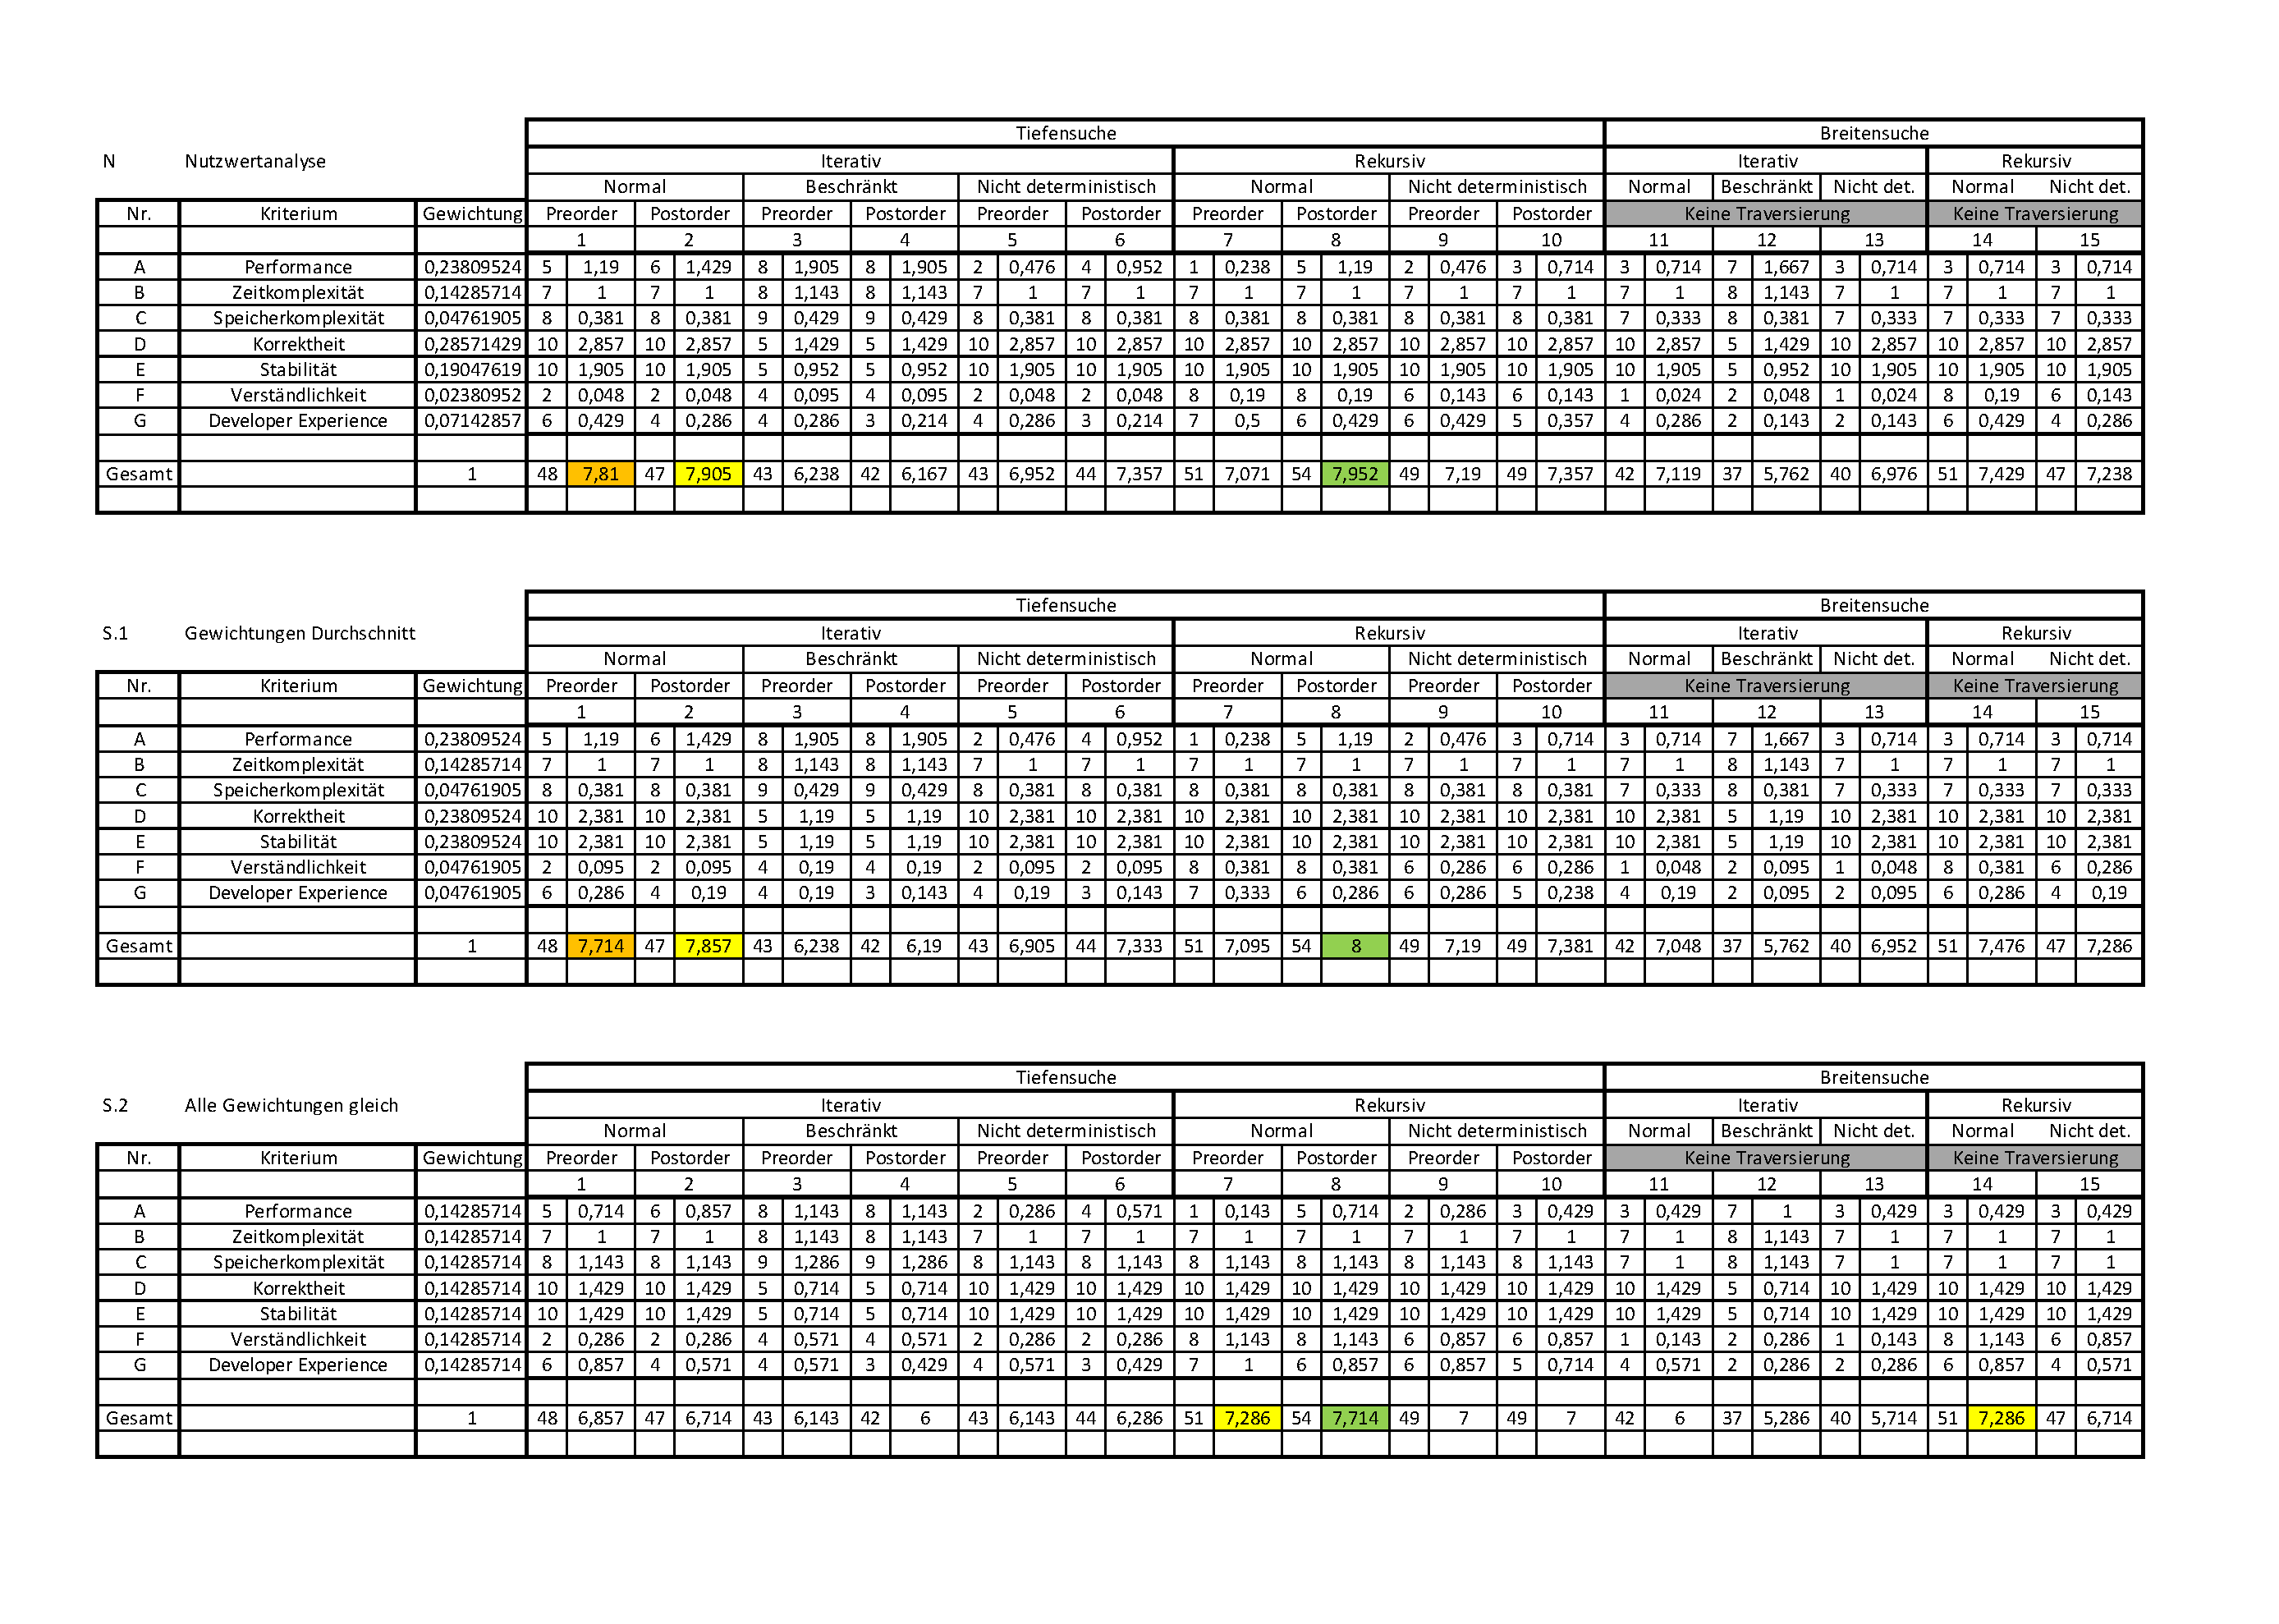
\includepdf[pages={1-3}]{Anhang/Nutzwertanalyse_Ergebnis.pdf}
%\appendix
%\include{Inhalt/05_Anhang/anhang}
%\clearpage
%\pagenumbering{Roman}  % römische Seitenzahlen für Anhang

\newpage
\end{document}
